
\section{Resoconti di verifica ed esiti delle revisioni}

In questa sezione vengono mostrati i valori delle metriche calcolate a termine del periodo di progettazione di dettaglio e codifica. Saranno mostrati sia i valori che rientrano nel range prestabilito sia quelli che non rientrano, nel secondo caso verranno segnalati come problemi nelle conclusioni che saranno divise per fasi.

\subsection{Metriche dei processi primari}
\subsubsection{percentuale di requisiti soddisfatti}

    \begin{figure}[H]
        \centering
        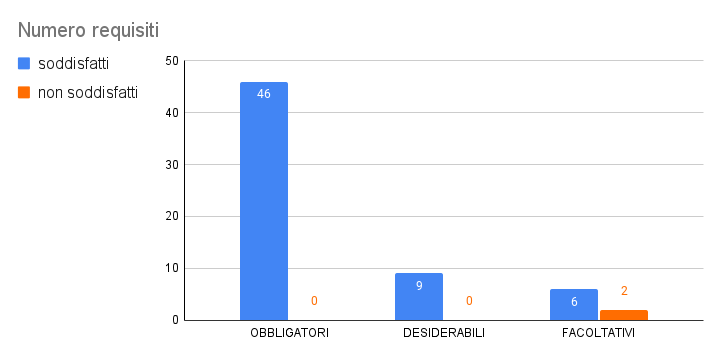
\includegraphics[width=13 cm]{source/sections/images/num-requisiti.png}
        \caption{Grafico dei requisiti}
    \end{figure}

    \begin{figure}[H]
        \centering
        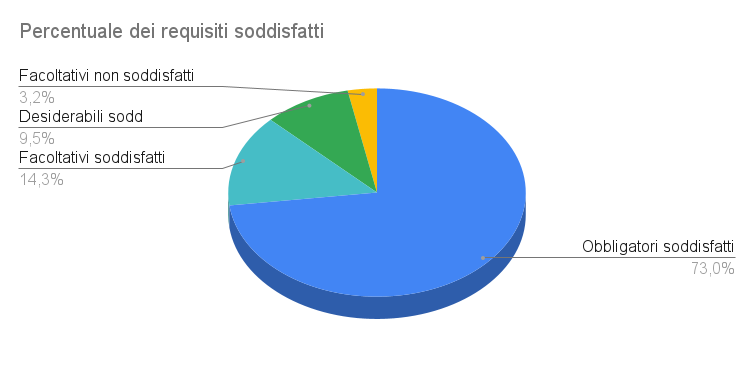
\includegraphics[width=13 cm]{source/sections/images/percentuale-requisiti.png}
        \caption{percentuale dei requisiti soddisfatti}
    \end{figure}

\subsubsection{Metriche di pianificazione}
    Le metriche di pianificazione che mostrano il rispettare dei costi e dei tempi sono stati calcolati in questa versione del documento in 6 gruppi denotati dalle seguenti sigle:
    \begin{itemize}
        \item \textbf{An}: Periodo di analisi, ovvero dal 26-11-2020 al 10-01-2021
        \item \textbf{CC}: periodo di consolidamento dei requisiti, ovvero dal 12-01-2021 al 18-01-2021
        \item \textbf{PA}: Progettazione architetturale, ovvero dal 19-01-2021 al 01-03-2021, che rappresenta la data progettata per la consegna
        \item \textbf{PAS}: Progettazione architetturale con consegna "a sportell0", ovvero dal 02-03-2021 al 09-03-2021, che rappresenta la data spostata con consegna il 10 marzo
        \item \textbf{PDC}: Progettazione di dettaglio e codifica, ovvero dal 10-03-2021 al 19-04-2021
        \item \textbf{VeC}: Verifica e collaudo, ovvero dal 20-04-20201 al 21-05-2021
    \end{itemize}
    
    
    \begin{longtabu} to \textwidth {| X[0.1,c m] | X[0.1,c m]| X[0.1,c m]| X[0.1,c m]| X[0.1,c m]| X[0.1,c m] |}
        \hline
        \rowcolor{header}
        \textbf{Fase} &
        \textbf{EV} &
        \textbf{PV} &
        \textbf{AC} &
        \textbf{SV} &
        \textbf{CV} \\
        \hline
        An & - & - & - & - & -  \\ 
        \hline
        CR & 734 & 734 & 650 & 0 & 84 \\
        \hline
        PA & 2588 & 3624 & 3439 & -1035 & -841\\
        \hline
        PAS & 1035 & 0 & 966 & 0 & 69 \\
        \hline
        PDC & 5935 & 5935 & 5935 & 0 & 0 \\
        \hline
        VeC & 3300 & 3300 & 3300 & 0 & 0 \\
        \hline 
        \end{longtabu}

        \begin{figure}
            \centering
            \makebox[\textwidth]{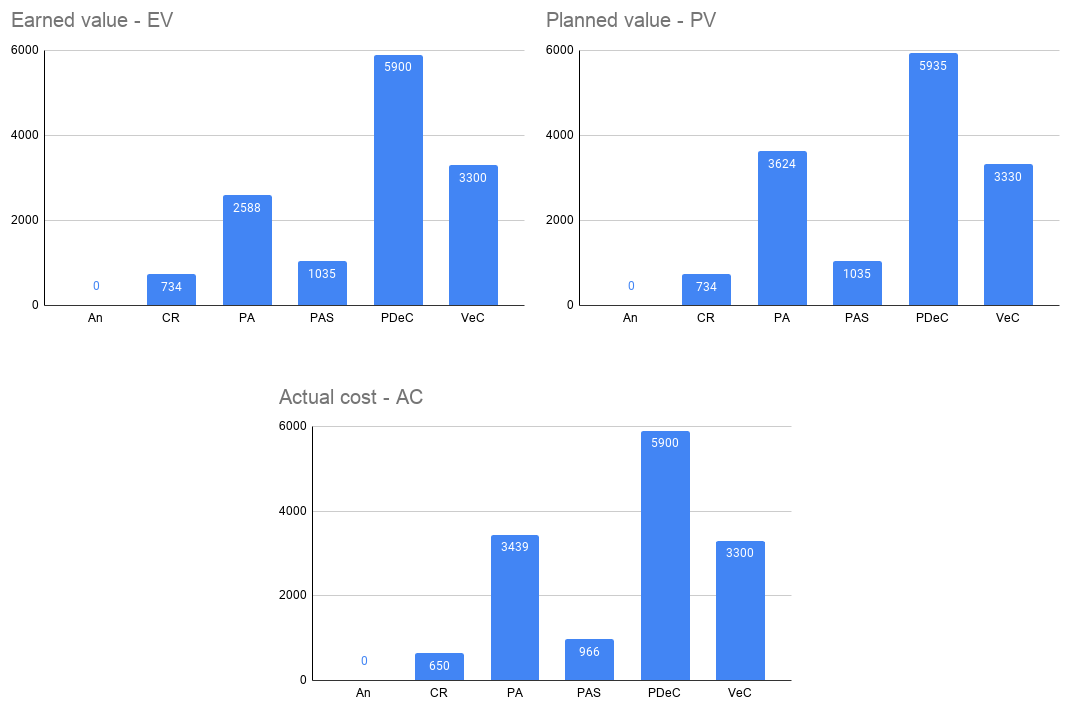
\includegraphics[width=18 cm]{source/sections/images/grafDiPianificazione.png}}
            \caption{Grafici dei valori di EV, AC e PV}\label{Y}
            \end{figure}


        \begin{figure}[H]
            \centering
            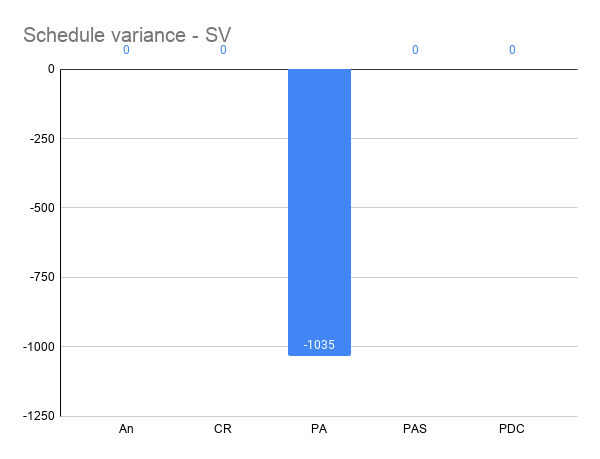
\includegraphics[width=12 cm]{source/sections/images/schedule_variance.png}
            \caption{Grafico dei valori dello Schedule variance}
        \end{figure}

        \begin{figure}[H]
            \centering
            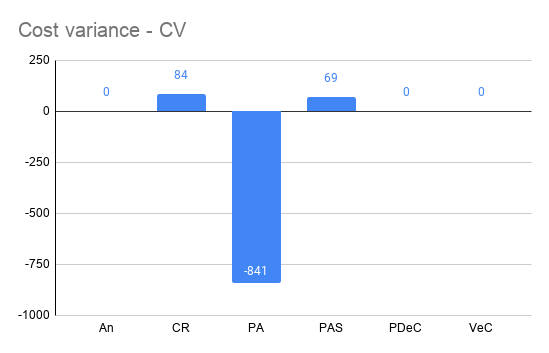
\includegraphics[width=12 cm]{source/sections/images/cost_variance.png}
            \caption{Grafico dei valori del Cost variance}
        \end{figure}


\newpage
\subsection{Metriche dei processi di supporto}
\subsubsection{Valori dell'indice di Gulpease}

Per ogni documento stilato è stato calcolato l'indice di Gulpease\glo{}. I valori sono dati dalla seguente tabella ed il rispettivo grafico con valore sufficiente >40 e valore ottimo >80.

\hphantom{}
\tabulinesep = 2mm % padding
\taburowcolors [1] 2{pari .. dispari} % colori delle righe

\begin{longtabu} to \textwidth {| X[0.2,c m]  | X[0.1,c m] | X[0.1,c m]| X[0.1,c m] | X[0.1,c m] |}
\hline
\rowcolor{header}
\textbf{Data del calcolo} &  
\textbf{Norme di Progetto} & 
\textbf{Analisi dei Requisiti} & 
\textbf{Piano di Qualifica} & 
\textbf{Piano di Progetto} \\
\hline

\multirow[c]{2}{*}{2020-12-03} & v0.1.0 & v0.2.4 & v0.2.1 & v0.1.0 \\
\cline{2-5} 
& 65 & 61 & 80 & 91 \\ 
\hline
\multirow[c]{2}{*}{2021-01-10} & v1.0.0 & v1.0.0 & v1.0.0 & v1.0.0 \\ 
\cline{2-5} 
 & 68 & 69 & 70 & 79 \\ 
\hline
\multirow[c]{2}{*}{2021-02-05}  & v1.0.1 & v1.0.5 & v1.0.2 & v1.0.2 \\ 
\cline{2-5} 
 & 75 & 74 & 64 & 83 \\ 
\hline
\multirow[c]{2}{*}{2021-02-20}  & v1.1.3 & v1.1.0 & v1.1.2 & v1.0.3 \\ 
\cline{2-5} 
 & 82 & 68 & 72 & 69 \\ 
\hline
\multirow[c]{2}{*}{2021-03-09} & v2.0.0 & v2.0.0 & v2.0.0 & v2.0.0 \\ 
\cline{2-5} 
 & 74 & 70 & 70 & 74 \\ 
\hline
\multirow[c]{2}{*}{2021-03-26}  & v2.0.2 & v2.1.0 & v2.0.1 & v2.0.3 \\ 
\cline{2-5} 
 & 73 & 69 & 70 & 73 \\ 
\hline
\multirow[c]{2}{*}{2021-03-4}  & v2.2.0 & v2.1.3 & v2.2.1 & v2.2.3 \\ 
\cline{2-5} 
 & 70 & 65 & 71 & 70 \\ 
\hline
\multirow[c]{2}{*}{2021-04-20}  & v3.0.0 & v3.0.0 & v3.0.0 & v3.0.0 \\ 
\cline{2-5} 
 & 68 & 64 & 72 & 68 \\ 
\hline
\end{longtabu}


\begin{figure}[H]
    \centering
    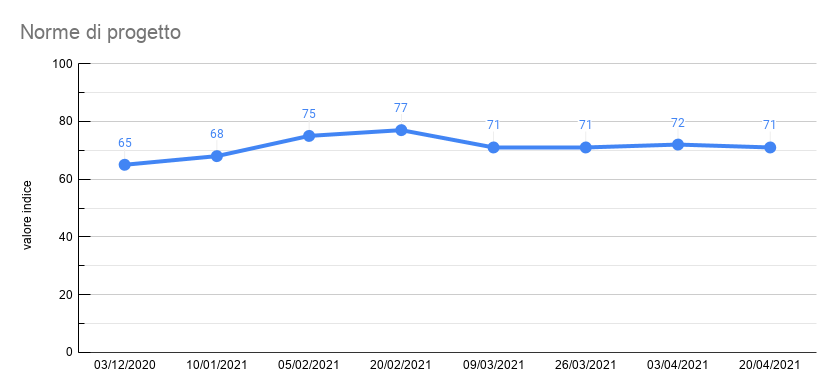
\includegraphics[width=13 cm]{source/sections/images/IdG_NdP.png}
    \caption{Indice di Gulpease - Norme di Progetto}
\end{figure}

\begin{figure}[H]
    \centering
    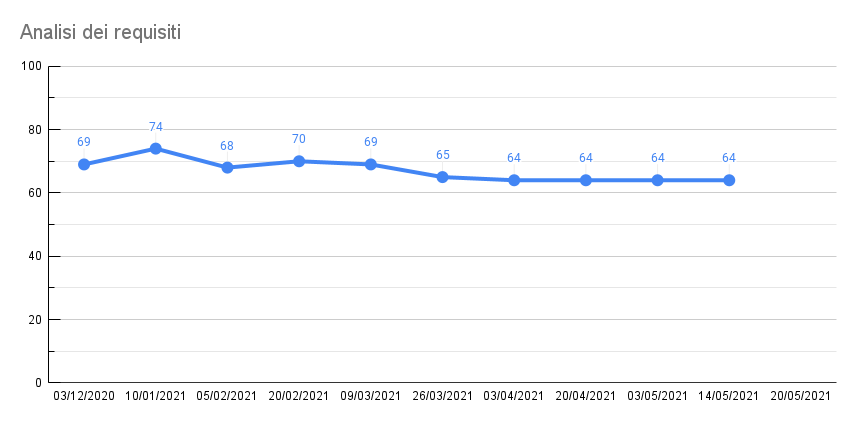
\includegraphics[width=13 cm]{source/sections/images/IdG_AR.png}
    \caption{Indice di Gulpease - Analisi dei Requisiti}
\end{figure}
\begin{figure}[H]
    \centering
    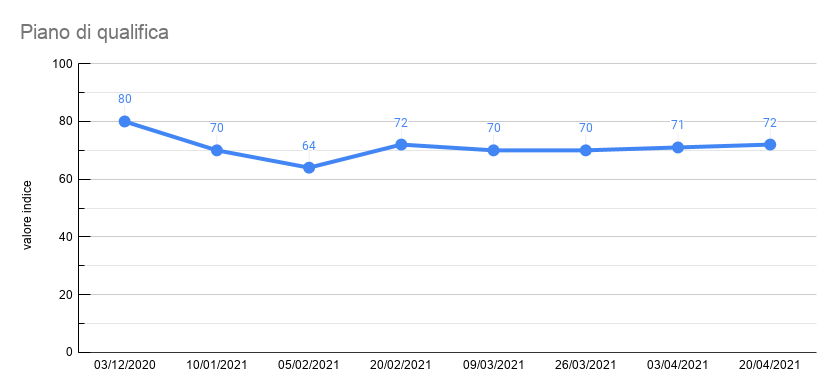
\includegraphics[width=13 cm]{source/sections/images/IdG_PdQ.png}
    \caption{Indice di Gulpease - Piano di Qualifica}
\end{figure}
\begin{figure}[H]
    \centering
    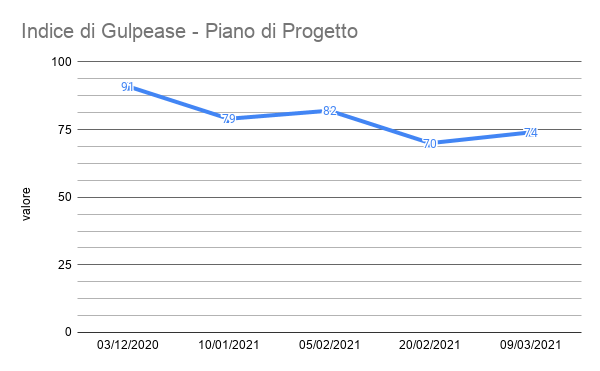
\includegraphics[width=13 cm]{source/sections/images/IdG_PdP.png}
    \caption{Indice di Gulpease - Piano di Progetto}
\end{figure}

\subsubsection{Errori ortografici}

Per quanto riguarda gli errori ortografici, oltre alla revisione fatta dai membri del gruppo, si è utilizzato anche lo spellchecker di Overleaf.

\newpage
\subsubsection{Percentuale di metriche soddisfatte}
    Per le metriche: Percentuale dei requisiti soddisfatti, complessità ciclomatica, sfin e sfout, alle quali sono stati determinati valori sufficienti e ottimi per ogni unità di calcolo,
    verranno considerate ottime se la maggior parte delle unità presenteranno valori ottimi. L'equivalente
    sarà considerato per i valori sufficienti e insufficienti. 


    \begin{longtabu} to \textwidth {| X[0.2,c m] | X[0.1,c m] | X[0.1,c m] |}
        \hline
        \rowcolor{header}
        \textbf{Metrica} &
        \textbf{Valore} &
        \textbf{Esito}\\
        \hline
        \hyperlink{subsubsection.5.1.1}{percentuale requisiti soddisfatti}& 74\% & insufficiente \\ 
        \hline
        \hyperlink{subsubsection.5.1.2}{Earned Value} & 5935 & ottimo  \\ 
        \hline
        \hyperlink{subsubsection.5.1.2}{Planned Value} & 5935 & ottimo  \\
        \hline
        \hyperlink{subsubsection.5.1.2}{Actual cost} & 5935 & ottimo  \\
        \hline
        \hyperlink{subsubsection.5.1.2}{Schedule variance Value} & 0 & ottimo  \\
        \hline
        \hyperlink{subsubsection.5.1.2}{Cost variance Value} & 0 & ottimo  \\
        \hline
        \hyperlink{subsubsection.5.2.1}{Errori ortografici} & 0 & ottimo  \\
        \hline
        \hyperlink{subsubsection.5.2.4}{Code coverage} & 12\% & insufficiente \\
        \hline
        \hyperlink{subsubsection.5.2.5}{Numero di test superati} & 57,6\% & insufficiente \\
        \hline
        \hyperlink{subsubsection.5.3.1}{Numero di click} & 2 & ottimo \\
        \hline
        \hyperlink{subsubsection.5.3.2}{Site depth} & 1 & ottimo \\
        \hline
        \hyperlink{subsubsection.5.3.3}Response time & 54,8 & ottimo \\
        \hline
        \hyperlink{subsubsection.5.3.4}{Complessità ciclomatica} & 99\% & ottimo \\
        \hline
        \hyperlink{subsubsection.5.3.5}{Facilità di comprensione} & 0.026 & insufficiente \\
        \hline
        \hyperlink{subsubsection.5.3.6}{sfin} & 59\% & Sufficiente \\
        \hline
        \hyperlink{subsubsection.5.3.6}{sfout} & 72\% & sufficiente \\
        \hline
        
        \end{longtabu}

        \begin{figure}[H]
            \centering
            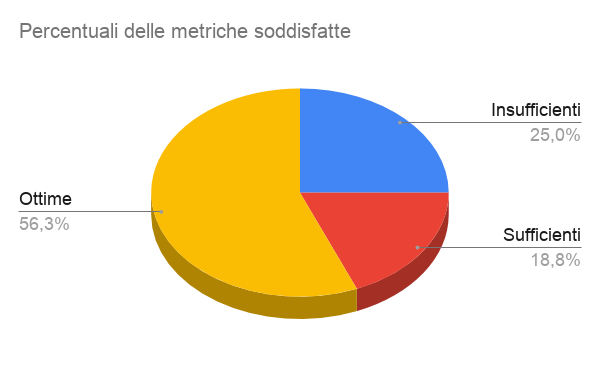
\includegraphics[width=14 cm]{source/sections/images/percentuale-metriche-soddisfatte.png}
            \caption{Grafico delle metriche soddisfatte}
        \end{figure}

\subsubsection{Code coverage}
    in questa fase del progetto didattico non si è data piena precedenza al numero di righe testate. E' stata comunque
    iniziata parzialmente una parte di testing. In seguito i valori del Code coverage calcolati dal 20 Marzo al 20 Aprile
    \begin{figure}[H]
        \centering
        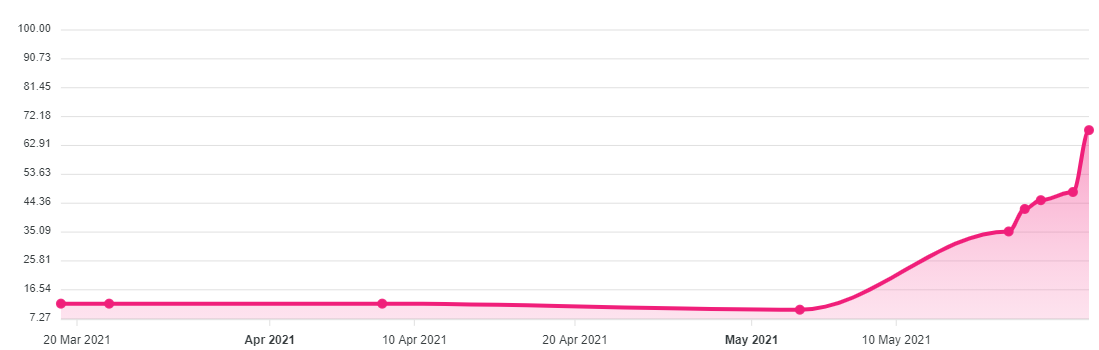
\includegraphics[width=16 cm]{source/sections/images/CodeCoverage.png}
        \caption{Grafico dei valori del Code coverage - GitHub}
    \end{figure}


\subsubsection{Numero di test superati}

    \begin{figure}[H]
        \centering
        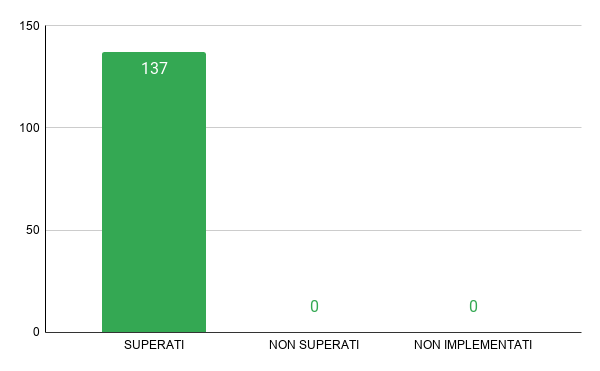
\includegraphics[width=10 cm]{source/sections/images/num-test.png}
        \caption{Grafico numero di test}
    \end{figure}

    \begin{figure}[H]
        \centering
        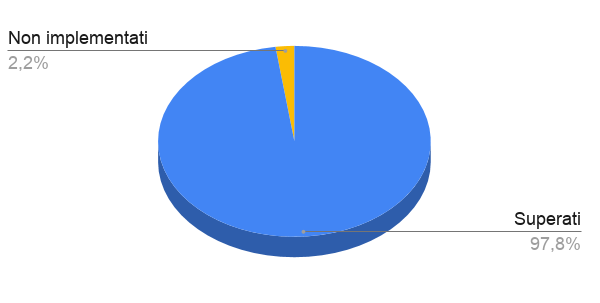
\includegraphics[width=10 cm]{source/sections/images/torta-test.png}
        \caption{Grafico della percentuale dei test}
    \end{figure}



\subsection{Metriche sulla qualità di prodotto}
\subsubsection{Correttezza dello scambio dei dati}
In accordo con il proponente del progetto la correttezza dello scambio dei dati, ovvero
il controllo su i possibili errori presenti nei dati, non è a carico del gruppo del progetto
ma verranno forniti dati pronti per l'elaborazione.
In conclusione la mterica può ritenersi con valore pari a zero e di conseguenza ottima.


\subsubsection{Numero di click}

\begin{longtabu} to \textwidth {| X[0.2,c m] | X[0.1,c m]| X[0.1,c m]| }
    \hline
    \rowcolor{header}
    \textbf{Task} &
    \textbf{Numero di click} &
    \textbf{Esito}\\
    \hline
    caricamento dati da csv & 2 & ottimo \\ 
    \hline
    caricamento dati da server & 3 & ottimo \\
    \hline
    visualizzare i dati & 3 + numero di features & sufficiente \\
    \hline 
    \end{longtabu}

\subsubsection{Site depth}
    L'applicazione web utilizza React e quindi fa in modo che la profondità del sito sia sempre pari ad 1, in quanto tutte le visualizzazioni vengono mostrate quando selezionate e calcolate sulla stessa pagina una alla volta

    
\subsubsection{Response Time}
    Il response time è stato calcolato su file csv di 150 record e i risultati in ms sono i seguenti:

    \begin{figure}[H]
        \centering
        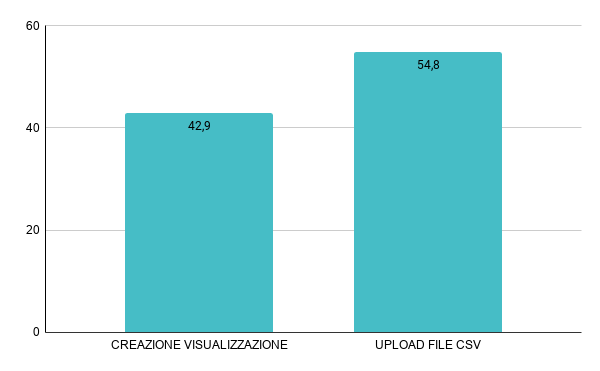
\includegraphics[width=10 cm]{source/sections/images/response-time.png}
        \caption{Grafico del response time}
    \end{figure}
    
\subsubsection{Complessità Ciclomatica}
    Nella seguente tabell e grafico si può vedere i valori della complessità cicolmatica divisi per valori:

        Come si può notare dal segeuente graico il numero di funzioni al di sotto della soglia per considerarsi ottime è pari al 97,82\%



    \begin{figure}[H]
        \centering
        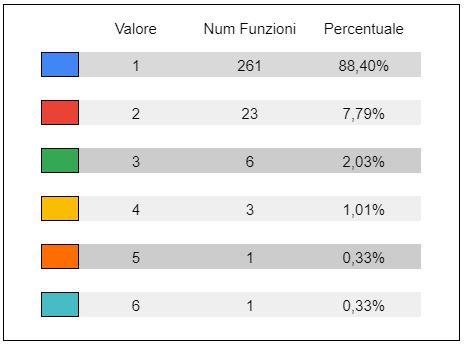
\includegraphics[width=10 cm]{source/sections/images/tabella_CC.JPG}
        \caption{Grafico della percentuale dei test}
    \end{figure}

    \begin{figure}[H]
        \centering
        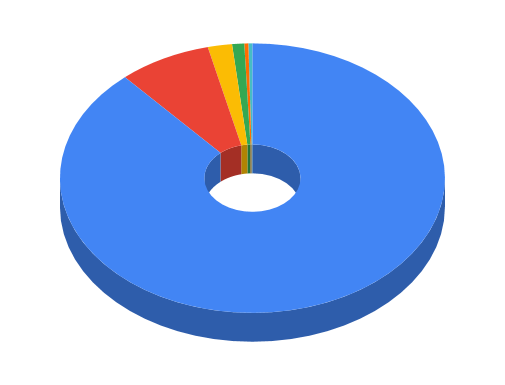
\includegraphics[width=10 cm]{source/sections/images/CC.png}
        \caption{Grafico della percentuale dei test}
    \end{figure}

    \subsubsection{Facilità di comprensione}

        \begin{figure}[H]
            \centering
            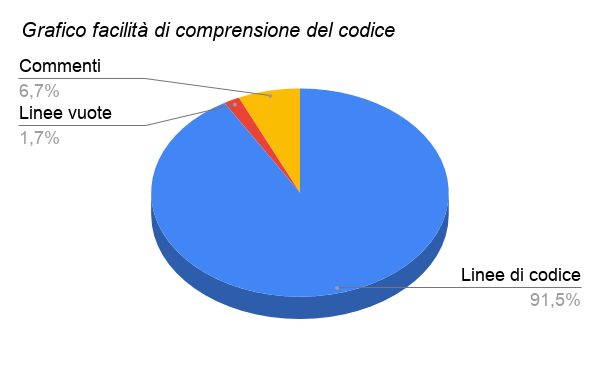
\includegraphics[width=10 cm]{source/sections/images/facilitaDelCodice.png}
            \caption{Grafico della facilità di comprensione}
        \end{figure}

    In seguito i grafici che mostrano l'andamento del numero di righe riguradnati, nel primo grafico il codice, e nel secondo
    le righe di commento e righe vuote

    \begin{figure}[H]
        \centering
        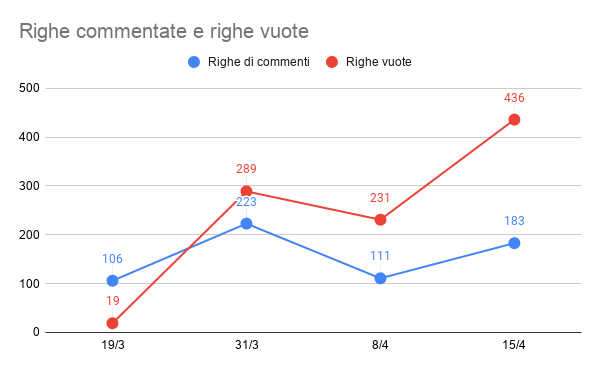
\includegraphics[width=10 cm]{source/sections/images/Valori-delle-righe.png}
        \caption{Grafico del numero di righe dei commenti e righe vuote}
    \end{figure}

    \begin{figure}[H]
        \centering
        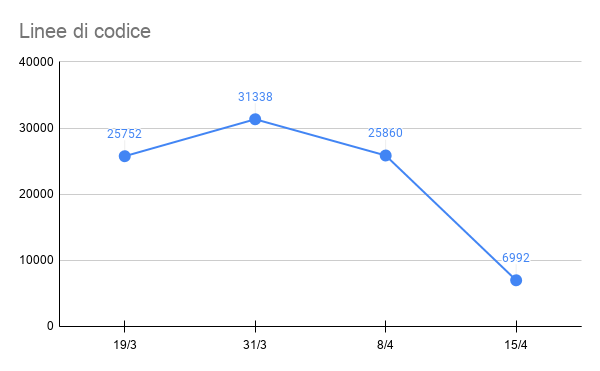
\includegraphics[width=10 cm]{source/sections/images/numCodice.png}
        \caption{Grafico del numero di righe di codice}
    \end{figure}

    \begin{figure}[H]
        \centering
        \includegraphics[width=10 cm]{source/sections/images/facilita_comprensione.png}
        \caption{Grafico della facilità di comprensione}
    \end{figure}

    I forti cambiamenti nell'andamento delle funzioni sono dati da un aggiornamento del progetto fatto in data
    9 Aprile (in fase di progettazione e collado), nel quale si è implementato un comando yarn che si preoccpa di creare la maggiorparte del
    codice CSS, che ha fatto scendere in modo drastico il numero di righe di codice del progetto effettivo.
\newpage
\subsubsection{SFIN and SFOUT}
    E' stato calcolato lo SFIN e SFOUT di tutti i 44 file del progetto. I risultati sono esposti nella seguente tabella:

    \begin{longtabu} to \textwidth {| X[0.1,c m] | X[0.1,c m] | X[0.1,c m] | X[0.1,c m] | X[0.1,c m] |}
        \hline
        \rowcolor{header}
        \textbf{Esito} &
        \textbf{IN} &
        \textbf{percentiale sul totale} &
        \textbf{OUT} &
        \textbf{percentuale sul totale} \\
        \hline
        Ottimo & 36 & 38,29\% & 32 & 34,04\% \\ 
        \hline
        Sufficiente & 46 & 51,11\% & 50 & 53,19\% \\ 
        \hline
        Insufficiente & 12 & 12,76\% & 12 & 12,76\% \\ 
        \hline

        \end{longtabu}

        \begin{figure}[H]
            \centering
            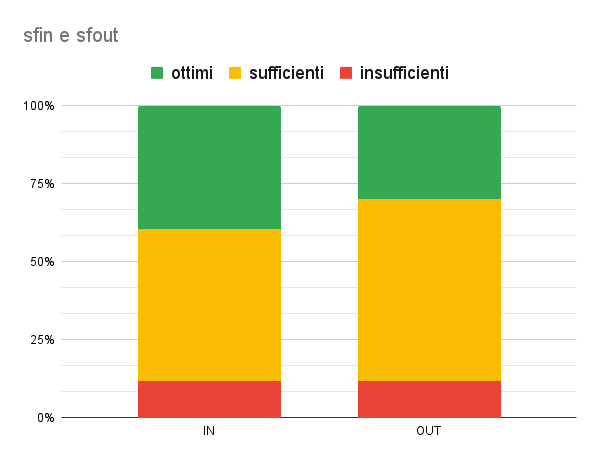
\includegraphics[width=13 cm]{source/sections/images/SfinSfout.png}
            \caption{Grafico dello sfin e sfout}
        \end{figure}

\newpage
\subsection{Conclusioni}

\subsubsection{Analisi}
Durante il periodo di analisi tutta la documentazione da presentare in ingresso alla revisione dei requisiti è stata sottoposta ad un'analisi meticolosa della struttura del documento, della chiarezza e degli errori ortografici. La verifica di ogni documento è stata svolta da 2 componenti del gruppo per assicurare il minor numero di errori possibili.
\newline
In conclusione dai valori raggiunti dal grafico e dalla tabella soprastanti, si evince un discreto lavoro di redattori e verificatori. In particolare sono stati utili il Piano di Qualifica e le Norme di Progetto per avere un punto di riferimento, sia agli analisti nella scrittura dei documenti, sia ai verificatori per controllare con metriche e con parametri oggettivi.

\subsubsection{Consolidamento dei requisiti}
Durante questo periodo si sono svolte le attività di consolidamento in anticipazione alla Revisione dei Requisiti.
In Conclusione i valori delle metriche in questo periodo sono tutte soddisfacenti ed alcune ottime, ciò indica il rispetto delle tempistiche ed una buona pianificazione da parte dei redattori del Piano di Progetto

\subsubsection{Programmazione architetturale}
Durante questo periodo si è individuata una soluzione architetturale del progetto e si è redatto il Proof of concept.
Gli scopi della programmazione architetturale non sono stati rispettati come si può vedere dalla Schedule variance con valore negativo, che indica un ritardo temporale da parte del gruppo.
Si è così deciso di sfruttare la consegna a sportello e recuperare la progettazione, recuperando così la perdita precedente. Si può vedere che la schedule variance del PAS è 0 che indica il rispetto delle tempistiche e l'Earned value della PAS corrisponde alle perdite del PA.
I valori del Cost variance leggermente positivi indicano una riuscita del rispetto dei costi e delle tempistiche ma senza un grande margine.
In Conclusione il gruppo è riuscito a recuperare grazie alla consegna a sportello, e non ha dovuto riconsegnare nella consegna successiva che avrebbe portato un ritardo e una perdita nei costi decisamente maggiore.

\newpage
\subsubsection{Proggettazione di dettaglio e codifica}

Durante questo periodo il progetto didattico ha preso forma. In particolare il gruppo ha posto l'accento sulla concretizzazione della product baseline, quindi dei design pattern, classi e attività necessarie alla codifica.
Infatti l'esito delle metriche inerenti a questi scopi è ottima il che conferma che una buona pianificazione aumenta la qualità del prodotto finale.
In particolare le metriche di pianificazione mostrano che non ci sono stati ritardi rispetto alla pianificazione e che si è rispettato il costo pianificato.
Le metriche della qualità di prodotto sono anch'esse tutte ottime, il che indica una buona direzione dell'andamento del progetto.

Una fonte di rischio di bassa qualità potrebbe essere il valore insufficiente di alcune metriche. Le metriche che hanno avuto un'esito insufficiente ovvero la percentuale dei requisiti soddisfatti, il code coverage e la facilità di comprensione del codice, saranno migliorate
nella fase finale di validazione e collaudo mediante una maggiore esecuzione di test e facendo leva sull'uso del ciclo di Deming, nel quale
vengono individuati i problemi, pianificate le soluzioni, verificare la soluzione e infine applicarla.
In particolare  verranno applicate le seguenti soluzioni:
\begin{itemize}
    \item \textbf{Facilità di comprensione del codice}: inserire commenti nelle parti di codice del progetto dove la complessità ciclomatica è superiore a 2
    \item \textbf{Code coverage}: aumentarne il valore nella fase di validazione e collaudo secondo la pianificazione della prossima fase  ponendo l'accento sui file con valori di FAN-in e FAN-out insufficienti
    \item \textbf{percentuale requisiti soddisfatti}: soddisfare il 26\% di requisiti rimanenti implementandoli nel progetto
\end{itemize} 
